\documentclass[10pt,letterpaper]{article}

\usepackage{cogsci}
\usepackage{pslatex}
\usepackage{amsmath}
\usepackage{amsfonts}
\usepackage{latexsym}
\usepackage{amssymb}
\usepackage{apacite}
\usepackage{graphicx}
\usepackage{caption}
\usepackage{subcaption}

\title{The Funny Thing About Incongruity: A Computational Model of Humor}
 
\author{{\large \bf Justine Kao (justinek@stanford.edu)} \\
  Department of Psychology \\
  Stanford, USA
  \AND {\large \bf Noah Goodman (ngoodman@stanford.edu)} \\
  Department of Psychology \\
  Stanford, USA
   \AND {\large \bf Roger Levy (rlevy@ucsd.edu)} \\
  Department of Linguistics \\
  UCSD, USA
  }


\begin{document}

\maketitle

\begin{abstract}


\textbf{Keywords:} 
Humor; language understanding; noisy channel; probabilistic models
\end{abstract}
\emph{``To preserve our marriage, my wife and I have a no pun relationship."}
\\
\section{Introduction}
Humor plays an essential role in human interactions. In a study on gender differences in desired characteristics of relationship partners, both men and women rated sense of humor as one of the most important qualities, above physical attractiveness and earning potential \cite{stewart2000sex}. Humor has important positive effects on children's development \cite{frank1989humor}, success in the work place \cite{duncan1990humor}, marital satisfaction \cite{ziv1989humor}, and coping with illness and traumatic events \cite{johnson2002use, gelkopf1996humor}. In this paper, we are interested in understanding how this fundamental and ubiquitous phenomenon works from the perspective of cognitive science. What makes something funny? How might the defining characteristics of humor shed light on the ways in which the mind processes and evaluates information?
\subsection{Incongruity theory of humor}
A leading theory in humor research is that incongruity is a necessary condition for humor \cite{veale2004incongruity, forabosco1992cognitive, mcghee1979humor, martin2007psychology, hurley2011inside}. As Veale (2004) states, ``Of the few sweeping generalizations one can make about humor that are neither controversial or trivially false, one is surely that humor is a phenomenon that relies on incongruity." Although there is disagreement in the literature about whether incongruity alone is sufficient, most theorists accept that humor requires perceiving a situation from different viewpoints and finding the subsequent interpretations of the same situation to be incompatible \cite{veatch1998theory, forabosco1992cognitive}. However, humor theorists' definitions of incongruity are often ambiguous and leave room for interpretation, making it difficult to test the role of incongruity empirically \cite{veale2004incongruity}. 

In this paper, we propose a computational model of humor that formalizes the concept of incongruity. We then test the role of incongruity in producing humorous sensations in the particular case of phonetically ambiguous sentences. 

\subsection{Computational humor}
Given the prevalence of humor in human communication, researchers in artificial intelligence have argued that computers should also be able to generate and detect humor in order to interact with humans more naturally and effectively \cite{mihalcea2006learning}. As a result, computational humor has made important progress and also received attention from popular press in the last decade (insert NYT citation here). However, most of the work in computational humor has focused either on utilizing joke-specific templates and schemata \cite{binsted1996machine, kiddon2011s}, or identifying linguistic features such as slang and alliteration that strongly predict humorous intent \cite{mihalcea2006learning, semantic2010}. The former type of studies is restricted to identifying jokes with a very specific format and structure, while the latter type falls short of testing or building upon deeper and more general theories of humor involving the management of incongruity. 

Our work moves beyond these two types of approaches and directly utilizes incongruence to identify humorous texts. Given that humor theorists view incongruity as an essential component of jokes, we examine whether human judgments of funniness can be predicted by the presence of incongruous interpretations of the same input. In particular, we aim to develop a formal model of linguistic humor that fits naturally into the framework of normal language processing. We propose that a noisy channel approach to language processing allows for multiple viewpoints on the same linguistic input and can thus naturally account for the possibility of incongruity. 

Our purposes for developing a formal model of linguistic humor are thus two-fold. First, we wish to formalize the concept of incongruity and test assumptions adopted by leading theories in humor research. Secondly, we aim to show that a noisy channel of language comprehension allows for the flexibility in context selection and interpretation that gives rise to sophisticated linguistic and social meaning such as humor. 

\section{The Noisy Channel and Incongruity}

In the section below, we describe the noisy channel model of sentence comprehension and its relevance to humor and incongruity. We present reasons for focusing on homophone puns and provide a high-level motivation for the model.

\subsection{Noisy channel models of sentence comprehension}
A central assumption in noisy channel models of sentence comprehension is that communication takes place under noisy conditions e.g. \cite{levy2008noisy}. As a result, not every piece of linguistic evidence faithfully represents the speaker's intended meaning. To achieve successful communication, a rational comprehender must use both the linguistic input itself as well as an understanding that the input may have been corrupted in order to infer the speaker's intended meaning. 

Previous work on noisy channel models of sentence comprehension has shown that such models are able to explain interpretation patterns of sentences with verb omission errors \cite{bergenverb}, garden path sentences \cite{levy2011integrating}, and even word order variation across languages \cite{gibsonnoisy}. These studies validate the idea that language comprehension is a rational process that incorporates uncertainty at the level of word-level input to affect sentence-level comprehension \cite{levy2008noisy}.

Given that sentence comprehension involves uncertainty about the linguistic input, a comprehender may rationally choose to consider only a subset of the input as relevant for uncovering the speaker's intended meaning. Since this rational process may lead the comprehender to consider multiple subsets of the input as equally relevant, these subsets can produce conflicting interpretations that result in a sensation of incongruity. The notion of incongruity thus fits naturally into a noisy channel model of sentence comprehension and can be formalized as such to explain its role in humor. 

Although the principle of a noisy channel can be applied to discourse and even non-linguistic input to explain longer jokes and visual puns \cite{abed1994visual}, in this paper we focus on a type of humorous input that is most directly related to existing work on noisy channel models of sentence comprehension: homophone puns.

\subsection{Homophone puns: a hare-y issue}
Writer and philosopher Henri Bergson defined a pun as ``a sentence or utterance in which two ideas are expressed, and we are confronted with only one series of words." Whether puns make you laugh or shake your head in despair, our ability to identify and understand puns reflects a distinctly human tolerance and even appreciation for incongruity. 

From a modeling perspective, homophone puns present an especially useful starting point for building probabilistic models of incongruity because competing interpretations of a pun are relatively shallow and easily represented. Consider the following sentence: 
\begin{itemize}
\item [] \emph{``The magician got so mad he pulled is hare out."} 
\end{itemize}
There are two interpretations of the sentence:
\begin{itemize}
\item[(a)] The magician got so mad he (idiomatically) pulled out the hair on his head.
\item[(b)] The magician got so mad he performed the trick of pulling a rabbit out of his hat.
\end{itemize}
This sentence is ambiguous due to the phonetically ambiguous word ``hare", which allows for two competing interpretations, \emph{hair} and \emph{hare}. These two interpretations can be easily approximated using the homonyms' lexical forms, ``hair" and ``hare." 

Importantly, ambiguity alone is not enough; plenty of sentences contain phonetically ambiguous words and yet are not funny. Instead, we propose that the detection of a pun hinges on successful identification of different contexts within a sentence or discourse that support different interpretations. Since subsets of this sentence simultaneously activate two incongruent interpretations of the same phonetic sequence, people find it more humorous than a similar sentence in which an alternative interpretation is not favored by any surrounding context. For example, \emph{``The professor got so mad he pulled his hair out}" is not a pun, just an unfortunate situation. 

We wish to capture the intuition that the magician and hare example produces humorous effects because:

\begin{itemize}
\item[(1)] ``hare" is a phonetically ambiguous word.
\item[(2)] Given the words ``mad," ``pulled," ``out," \emph{hair} is the most probable interpretation of ``hare."
\item[(3)] Given the word ``magician," \emph{hare} is the most probable interpretation of ``hare."
\item[(4)] From (2) and (3), given the full sentence, \emph{hair} and \emph{hare} are equally and highly probable interpretations.
\end{itemize}

In other words, focusing on different subsets of a sentence results in different highly probable interpretations. Based on this intuition, our model adopts a noisy channel model approach that probabilistically selects two subsets of a sentence as contexts and ignores the remaining words. The model then separately computes the probabilities of interpretations of the ambiguous word given the two selected contexts. Motivated by the incongruity theory of humor, we predict that sentences in which two sub-contexts produce very different meaning distributions for the ambiguous word are more likely to be funny. We present our model more formally in the following section.


\section{Model}
Suppose a sentence $S$ is composed of words $w = \{w_1, w_2, \dots ,w_n\}$ and $h$. $h$ is a phonetically ambiguous word that has two homophone interpretations or meanings, $m_1$ and $m_2$. 

We assume that at a given point in time, only a subset of words in $w$ contributes to the interpretation of $h$. This is a noisy model in which listeners assume that speakers have a probability of uttering spurious or incorrect words that do not contribute to the interpretation of the ambiguous word $h$. Suppose each word $w_i$ has a probability $p_i$ of being ``spurious" or ignored. Note that $p_i$ can be a function of the distance between $w_i$ and $h$, with $p_i \propto$ distance between $w_i$ and $h$.

Under this framework, the probability of a certain subset of words context $C = \{c_{1}, c_{2}, \dots, c_{l}\}$ being ``in focus" is given by the following:
$$
P(C) = \prod_{j=1} ^ {m} (1 - p_{j})
$$
Furthermore,
\[
   \left\{ 
  \begin{array}{l}
   P(m_1, C) = P(m_1 | C) P(C)\\
   P(m_2, C) = P(m_2 | C) P(C)\\
  \end{array} \right.
\]

At any given time, two contexts compete with each other to determine the correct interpretation. This allows us to formalize incongruity by measuring the difference between the interpretations given by the two contexts. The larger the difference, the larger the incongruity, and thus the funnier the sentence. 

\subsection{Computing interpretation probabilities}
Suppose a context $C = \{c_{1}, c_{2}, \dots, c_{l}, h\}$ is in focus. We assume that $h$ itself (the written and observed word) can also be in $C$. To compute the probability of an interpretation of $h$ given $C$, we assume a generative model in which $C$ is generated independently given an interpretation $m$. By Bayes' Theorem,
$$
P(m | c_1, c_2, \dots, c_l, h)  = P(m) \frac{P(h | m)}{P(h)}\prod_i^l \frac{P(c_i | m)}{P(c_i)}
$$
\subsection{Computing incongruity}
Given the derivations above, we compute the interpretation probabilities of $h$ for any two contexts $C_1$ and $C_2$.

We can thus compute the interpretation distributions of $m$ given $C_1$ and $C_2$, denoted as the following: $C_1(m)$ and $C_2(m)$. Since $C_1(m)$ and $C_2(m)$ are two probability distributions, we can compute their distance using standard measures from information theory. Since incongruity between two contexts should be symmetric, we select symmetrised KL divergence, defined as the following:
$$
D_{KL}(P || Q) + D_{KL}(Q || P) = \sum_x \bigg ( \ln \frac{P(x)}{Q(x)} P(x) +  \ln \frac{Q(x)}{P(x)} Q(x) \bigg )
$$
Given two contexts $C_1$ and $C_2$, the distance in meaning distributions of $h$ is given by the following:
$$
\sum_k \bigg ( \ln \frac{P(m_k | C_1)}{P(m_k | C_2)} P(m_k | C_1) +  \ln \frac{P(m_k | C_2)}{P(m_k | C_1)} P(m_k | C_2) \bigg )
$$
Summing over all possible context combinations, our formal measure of a sentence's incongruity is the sum of the symmetrised KL distance for each context combination weighted by the probability of selecting those contexts:
$$
 \sum_{C_1, C_2} P(C_1) P(C_2) \sum_k \bigg ( \ln \frac{P(m_k | C_1)}{P(m_k | C_2)} P(m_k | C_1) +  \ln \frac{P(m_k | C_2)}{P(m_k | C_1)} P(m_k | C_2) \bigg )
$$
Under this framework, $m_i$ can be any existing meaning. However, for simplicity, we assume that given the written word $h$ in $C_1$ and $C_2$, $P(m_k | C_1) = P(m_k | C_2) = \epsilon$ for all $m_k$ that are not exact homophones of $h$ and can be ignored. Thus we are only interested in interpretations $m_1$ and $m_2$, which are exact homophones of the written word $h$.

By combining a noisy channel model of language processing, a Bayesian model for meaning distributions, and a standard information theoretic measure of symmetrised KL divergence, our model presents a formal measure of incongruity to test the incongruity theory of humor.  

\section{Evaluation}
We evaluate our model on a set of $160$ sentences, consisting of $40$ puns, $80$ control non-pun sentences that match the puns in containing the same phonetically ambiguous words, and $40$ ``de-punned" control sentences that are matched with the puns but with certain manipulations described below. We evaluate our model based on how well it predicts people's funniness ratings of these sentences.
\subsection{Materials}
We selected $40$ pun sentences from a large collection of puns on a website called �Pun of the Day,� which contains over a thousand original puns. Puns were selected such that the ambiguous item is a single phonetically ambiguous word, and such that no two puns in the collection have the same ambiguous item.

The $80$ non-pun sentences were chosen to match each pun sentence on its ambiguous word as well as the alternative homophone. The sentences were taken from an online version of Heinle's Newbury House Dictionary of American English (http://nhd.heinle.com/). We selected sample sentences included in the definition of the homophone word. This design ensured that puns and non-pun sentences contain the same phonetically ambiguous words, a control that was not used in previous work on automatic humor recognition.

We also constructed $40$ sentences to be minimally different from the pun sentences, which we will call de-punned sentences. An undergraduate research assistant who was blind to the hypothesis and model was asked to replace one word in each of the pun sentences (without changing the homophone word itself) so that the sentence still makes sense but is no longer a pun. This resulted in sentences that were only one word different from the pun sentences. Below are example sentences from each category.\\\\
\begin{tabular}{| l | l |}\hline
\textbf{Type} & \textbf{Example}} \\\hline
Pun & ``The magician got so mad he pulled his hair out." \\
De-punned & ``The teacher got so mad he pulled his hair out."\\
Normal & ``The hare ran rapidly across the field."\\
Normal & ``Some people have lots of hair on their heads."\\\hline
\end{tabular}\\\\

\subsection{Human ratings of semantic relatedness}

\begin{figure}[t]
\scalebox{0.44}{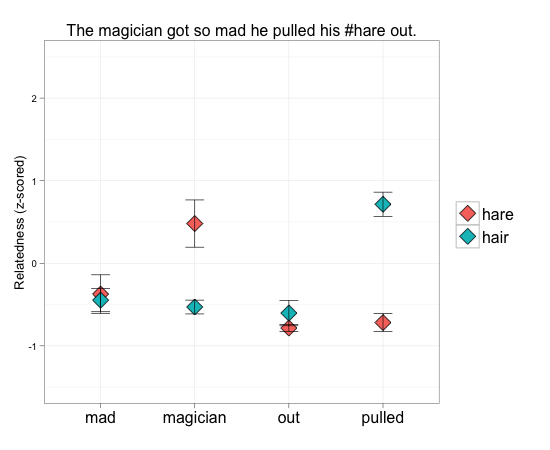
\includegraphics{Plots/hare_pun.png}}
\caption{Relatedness of word pairs in example pun.}
\end{figure}


As described in the model section, in order to compute interpretation probabilities of the homophone word given different contexts, we need the conditional probabilities of each word in the context given the homophone word $P(c_i | m)$. However, $P(c_i | m)$ is difficult to obtain through corpora (due to data sparsity) as well as through empirical measures of association strength (due to the large number of subjects one must recruit in order to obtain a good estimation of subjects' likelihood of thinking of $c_i$ given $m$). As a result, we chose to approximate $P(c_i | m)$ using empirical measures of the semantic relatedness between $c_i$ and $m$, denoted as $R(c_i, m)$. We use $R(c_i, m)$ as an approximate measure of point wise mutual information between $c_i$ and $h$, defined as follows:
$$
R(c_i, m)  = pmi(c_i, m)= {\log \frac{P(c_i, m)}{P(c_i)P(m)}}
$$
With the proper substitutions, the derivation of $P(m | c_1, \dots, c_l, h)$ can be reduced to the following:
$$
\log P(m | c_1, \dots, c_l, h)
= \log P(m) + R(h, m) + \sum_i^l R(c_l, m) 
$$

To obtain $R(c_i, m)$ for each of the words $c_i$ in the $160$ sentences, we recruited $200$ subjects on Amazon's Mechanical Turk to rate distinct word pairs on their semantic relatedness. Function words were removed from the sentences, and the remaining words were paired with each of the interpretations of the homophone sequence (e.g., ``magician" and ``hare" is a legitimate word pair, as well as ``magician" and ``hair"). This resulted in $1460$ distinct word pairs. Each subject saw $146$ pairs of words in random order and were asked to rate how related each word pair is from $1$ to $10$. The average split-half correlation of the relatedness ratings was $0.916$. 

Figure 1 and 2 show the relatedness of content words in the sentence with the two homophone interpretations. We see that in the pun sentence, the word ``magician" is rated as significantly more related to ``hare" than it is to ``hair", while the word ``pulled" is rated as significantly more related to ``hair" than it is to ``hare." On the other hand, all words in the non-pun example are significantly more related to the word ``hare" than to ``hair."

Figure 3 shows the average relatedness ratings of words and the two homophone interpretations across the three types of sentences. We see that in pun sentences, the average relatedness of words to the two homophone interpretations are roughly equivalent. In the non-pun sentences, the average relatedness of words to the observed homophone is significantly higher than to the alternative homophone. This analysis of human ratings of relatedness supports the intuition on which our model is based that funnier sentences are those in which different contexts support incongruous interpretations of the homophone.

\begin{figure}[t]
\scalebox{0.45}{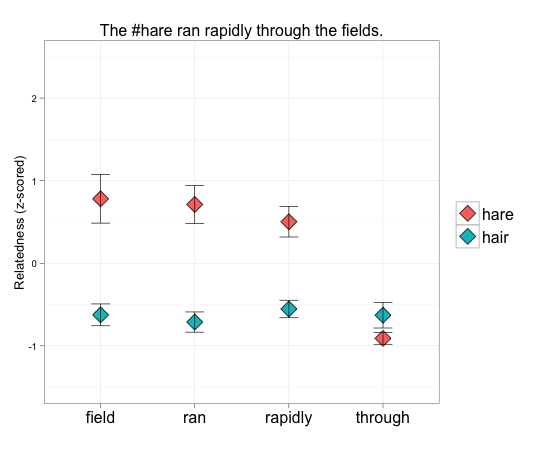
\includegraphics{Plots/hare_nonpun.png}}
\caption{Relatedness of word pairs in example non pun.}

\end{figure}

\begin{figure}[t]
\scalebox{0.45}{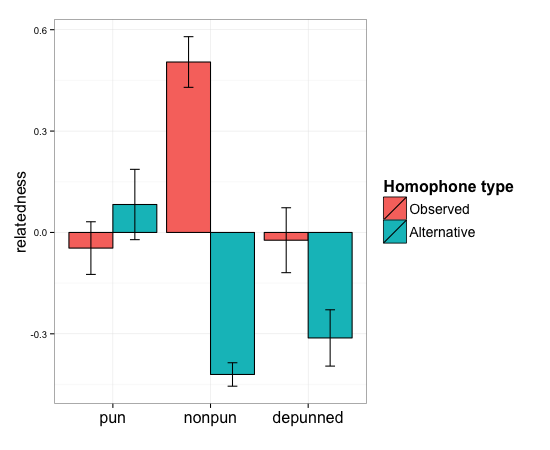
\includegraphics{Plots/ave_relatedness.png}}
\caption{Average relatedness ratings across sentence types}
\end{figure}

\subsection{Human Ratings of Funniness}
We obtained funniness ratings of the sentences from a separate pool of subjects on Amazon's Mechanical Turk. $100$ subjects rated the sentences on funniness. Split-half correlation was ~ Figure 4 shows the average funniness ratings of puns, non-puns, and de-punned sentences. We see that pun sentences are rated as significantly funnier as de-punned sentences, and de-punned sentences are rated as significantly funnier than non-pun sentences.
\begin{figure}[h]
\scalebox{0.45}{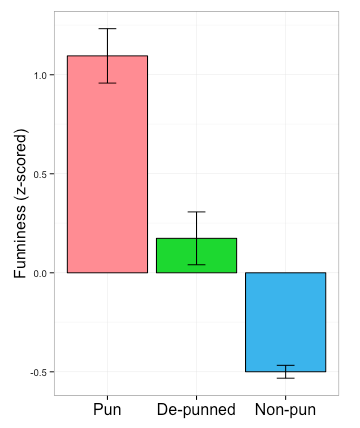
\includegraphics{Plots/ave_funniness.png}}
\caption{Average funniness ratings across sentence types}
\end{figure}


\section{Results}
Show incongruity measures across sentence categories. Show model predictions of funniness based on incongruity measures and correlation with human ratings of funniness. 

\section{Discussion}
Show how our model is directly motivated by incongruity theories of humor and provides a useful formalization that predicts subjective ratings of funniness. Discuss how it is able to select contexts that give maximal incongruity and maximal justification, which can tell us \emph{why} a pun is funny in addition to when it is funny. Describe its advantages over previous work on computational humor. Describe potential applications and generalizations to other forms of humor. 

\section{Acknowledgments}


\section{References}

\bibliographystyle{apacite}

\setlength{\bibleftmargin}{.125in}
\setlength{\bibindent}{-\bibleftmargin}

\bibliography{pun_bib}


\end{document}
